% !TEX options=--shell-escape
\documentclass [12pt]{article} 

\usepackage{amsmath}
\usepackage{amsthm}
\usepackage{amssymb}
\usepackage{graphicx} 
\usepackage{float}
\usepackage{multirow}
\usepackage{xcolor}
\usepackage [ruled,vlined,commentsnumbered,titlenotnumbered]{algorithm2e} \usepackage{array} 
\usepackage{booktabs} 
\usepackage{url} 
\usepackage{parskip} 
\usepackage [margin=1in]{geometry} 
\usepackage [T1]{fontenc} 
\usepackage{cmbright} 
\usepackage [many]{tcolorbox} 
\usepackage [colorlinks = true,
            linkcolor = blue,
            urlcolor  = blue,
            citecolor = blue,
            anchorcolor = blue]{hyperref} 
\usepackage{enumitem} 
\usepackage{xparse} 
\usepackage{verbatim}
\usepackage{listings}
\usepackage{xcolor}
\usepackage{csquotes}
\usepackage[cache=false]{minted}
\usepackage{mdframed}
\usepackage{tikz}
\usepackage{algpseudocode}
\usepackage{wrapfig}

\usetikzlibrary{shapes.symbols}
\newtheorem{theorem}{Theorem}

\BeforeBeginEnvironment{minted}{\begin{mdframed}}
\AfterEndEnvironment{minted}{\end{mdframed}}

\DeclareTColorBox{Solution}{}{breakable, title={Solution}}
\DeclareTColorBox{Solution*}{}{breakable, title={Solution (provided)}}
\DeclareTColorBox{Instruction}{}{boxrule=0pt, boxsep=0pt, left=0.5em, right=0.5em, top=0.5em, bottom=0.5em, arc=0pt, toprule=1pt, bottomrule=1pt}
\DeclareDocumentCommand{\Expecting }{+m}{\textbf{[We are expecting:} #1\textbf{]}}
\DeclareDocumentCommand{\Points }{m}{\textbf{(#1 pt.)}} 
\newcommand{\hint }[1]{\noindent{[\textbf{HINT:} \em #1 \em ]}} \newcommand{\pts }[1]{\textbf{(#1 pt.)}} 

\begin{document} 

{\LARGE \textbf{COMP 285 (NC A\&T, Spr `22)}\hfill \textbf{Homework 10} } 
\vspace{1em} 
\begin{Instruction} 

\paragraph{Due.} Friday, April 29th, 2022 @ 11:59 PM!
\end{Instruction}

\vspace{1em} 
\begin{Instruction} \paragraph{Homework Expectations:} Please see \href{https://www.comp285.ml/homework/#general-homework-information}{Homework}.
\end{Instruction}

\vspace{1em} 
\begin{Instruction} 

\paragraph{Exercises} The following questions are exercises. We encourage you to work with a group and discuss solutions to make sure you understand the material.

\paragraph{Points} This assignment is graded out of 50 points. However, you can get up to 60 points if you complete everything. These are not bonus points, but rather points to help make-up any parts you miss.

\end{Instruction} 

\begin{centering}
\section*{Fun with MSTs, Flows, and Cuts}
\end{centering}

\begin{Instruction}

\paragraph{Written Problems} The following questions are to be submitted in written/typed form to gradescope.

\end{Instruction}

\section{Learning for Fun \Points{0}}
Watch 1 (<30 minute video) or read 2 before you start the following two questions:

\begin{enumerate}
  \item If you prefer a lecture format, this is a \href{https://www.youtube.com/watch?v=wU6udHRIkcc}{really good video resource} (as a general note, this person's lectures are high quality across the board). Slight terminology differences in this video from the HW and textbook: he uses “weighted union” which is similar to the “union by rank”, and he says “collapsing find” which is essentially “path compression”.
  \item If you prefer a written resource, Ch 21 in the CLRS textbook is fully dedicated to the topic. You can skip over the exercises and detailed math proofs to understand the main ideas, and they are very similar to the ideas explained in the video.
\end{enumerate}

\pagebreak
\section{Understanding Kruskal's Algorithm \Points{8}}
In class, we showed an abbreviated version of Kruskal's pseudocode. The actual pseudocode looks like this:

\begin{verbatim}
algorithm kruskal(G, w)
  Input: A connected undirected graph G = (V, E) with edge weights w(u, v) 
    for all (u,v) in E
  Output: A minimum spanning tree defined by the edges X

  for all u in V:
    makeset(u)
  X = {}
  Sort the edges E by weight
  for all edges {u, v} in E, in increasing order of weight:
    if find(u) != find(v):
      add edge {u, v} to X
      union(u, v)
  return X
\end{verbatim}

Recall during the Kruskal's lecture (\href{https://www.comp285.ml/lectures/#kruskal-s-algorithm-and-max-flow}{Lecture 32}) how we would make sure that adding an edge between two nodes would not create a cycle. A data structure called "Disjoint Sets" allow us to do this efficiently by keeping track of / updating a "set" for each connected component.

We have 3 functions related to Disjoint Sets:

\begin{enumerate}
  \item \texttt{makeset}(x), which takes in a node x and creates a new set with just x in it.
  \item \texttt{find}(x), which takes in a node and returns which set it belongs to.
  \item \texttt{union}(x, y), which takes in two sets, and combines them into one big set.
\end{enumerate}

\subsection{\Points{2}}
How many times will we call \texttt{makeset} within Kruskal's? Put your answer in terms of $n = |V|$ and $m = |E|$.

\Expecting{A mathematical expression using $n$ and $m$.}

\subsection{\Points{2}}
How many times will we call \texttt{find} within Kruskal's? Put your answer in terms of $n = |V|$ and $m = |E|$.

\Expecting{A mathematical expression using $n$ and $m$.}

\subsection{\Points{2}}
How many times will we call \texttt{union} within Kruskal's? Put your answer in terms of $n = |V|$ and $m = |E|$.

\Expecting{A mathematical expression using $n$ and $m$.}

\subsection{\Points{2}}
Describe using your own words why \texttt{find}(u) != \texttt{find}(v) is the same as "if this edge doesn't cause a cycle".

\Expecting{One sentence explaining the above.}


\pagebreak
\section{Disjoint-Set Data Structure \Points{8}}
Now here's the code for the Disjoint Set functions above:

\begin{verbatim}
algorithm makeset(x)
  Input: a graph node x
  Output: modify x such that it has a "rank" and a "parent"

  x.rank = 0
  x.parent = x

algorithm find(x)
  Input: a graph node x
  Output: the ancestor

  if x != x.parent
    x.parent = find(x.parent)
  return x.parent

algorithm union(x, y)
  Input: graph nodes x and y
  Output: modify x and y so that they are now connected in the same "set"

  x = find(x)
  y = find(y)

  if x.rank > y.rank
    y.parent = x
  else
    x.parent = y
    if x.rank == y.rank
      y.rank = y.rank + 1
\end{verbatim}


\subsection{\Points{2}}
Suppose we make the following sequence of calls: `\texttt{makeset}(A); \texttt{makeset}(B); \texttt{makeset}(C); \texttt{makeset}(D); \texttt{union}(C, D); \texttt{union}(A, B); \texttt{union}(B, D);`. Draw what the set(s) look like at this point (either a picture or text representation is fine).

\Expecting{Include an image or text representation of what the data structure looks like.}

\subsection{\Points{2}}
You call `\texttt{find}(x)` on the above and it takes multiple recursive calls, then you call `\texttt{find}(x)` again on the same node and it takes fewer. What is `x`? This phenomena is called "path compression".

\Expecting{A short explanation of what `x' stands for.}

\subsection{\Points{2}}
Draw what the set(s) look like after the additional `\texttt{find}` calls. 

\Expecting{Include an image or text representation of what the data structure looks like.}

\subsection{\Points{2}}
What does rank signify for each node?

\Expecting{A short explanation of what the `rank' represents}.


\pagebreak
\section{Network Flow Cuts \Points{14}}

An \textbf{s-t cut} of a flow network is a partitioning of nodes into two groups, one which contains the source $s$ and the other which contains the sink $t$. 

\begin{figure}[h!]
\centering
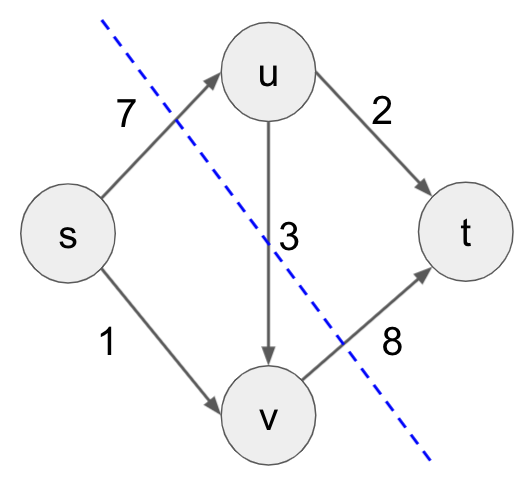
\includegraphics[scale=0.5]{cut-example.png}
\caption{An example of an s-t cut.}
\label{fig:cut_example}
\end{figure}


The image in Figure \ref{fig:cut_example} represents the cut $\{s, v\} / \{u, t\}$. The \textbf{cut capacity} is the sum of all edge capacities that \textbf{go from the set containing s to the set containing t}. So the cut capacity shown above is $7 + 8 = 15$ (note that we do not include $3$).

\subsection{\Points{9}}

Define all 4 s-t cuts in the graph above and calculate their capacities. The \href{https://en.wikipedia.org/wiki/Max-flow_min-cut_theorem} states that the max flow in a network is equal to the capacity of the $s-t$ cut with minimum capacity. Using this, what is the max flow of this network?

\Expecting{The 4 s-t cuts along with their capacities and the value of the max flow.}


\subsection{\Points{5}}

Find and list flow values for each edge that will give this max-flow. What do you notice about the flows of the edges along the minimum s-t cut? Use this observation to explain why the max-flow min-cut theorem makes intuitive sense.

\Expecting{Flows for each edge and a short explanation of why the max-flow min-cut theorem makes sense.}


\pagebreak
\section{Negative Prim? \Points{5}}
\label{sec:last}
We want to now consider a similar algorithm to Prim's called Negative-Prim for computing minimum spanning tree in graphs with negative edge weights.

This algorithm adds some number to all of the edge weights to make them all nonnegative, then runs Prim's algorithm on the resulting graph, and argues that the Minimum Spanning Tree in the new graph are the same as the MST in the old graph. You can assume that all the edge weights are unique integers.

\begin{verbatim}
Negative-Prim(G, s):
  minWeight = minimum edge weight in G
  for e in E: # iterate through all edges in G
    modifiedWeight(e) = w(e) - minWeight
    modifiedG = G with weights modifiedWeight
  T = Prim(modifiedG, s) # run Prim's algorithm starting from s
  update T with edges that corresponds to graph G
  return T
\end{verbatim}

\Expecting{Either an informal explanation of why Negative-Prim computes the
correct MST, or a counter-example of an undirected graph with negative edge weights where
Negative-Prim does not output}


\section*{Submitting the Assignment}

The assignment should be submitted through \href{https://www.gradescope.com/courses/350304}{Gradescope}.

The "Homework 10: Fun with MSTs, Flow, and Cuts" assignment is the written portion, for which you should submit a \textbf{typed} response to questions 1-\ref{sec:last}. Each response should clearly be marked with its corresponding number. You are free to use the provided templates, print the questions and write your answers, or to simply type your responses on a blank document (whatever works for you).


\end{document} 